\documentclass[11pt]{article}
\usepackage[margin=1.1in]{geometry}
\usepackage{amsmath, amssymb, amsthm}
\usepackage{natbib}
\usepackage{booktabs}
\usepackage{graphicx}
\usepackage[colorlinks=true, citecolor=blue, linkcolor=blue, urlcolor=blue]{hyperref}

\newtheorem{proposition}{Proposition}
\newtheorem{lemma}{Lemma}
\newtheorem{corollary}{Corollary}
\newtheorem{assumption}{Assumption}
\theoremstyle{remark}
\newtheorem{remark}{Remark}

\title{The Intelligence Cost of Surveillance\thanks{Draft: June 2026. Companion to ``Speaking in Code: How Surveillance Suppresses Coordinated Dissent.'' Replication code and data: see repository. I thank [advisor, seminar participants] for comments.}}
\author{Khaled Eltokhy\\ \small Department of Economics, The Graduate Center, CUNY}
\date{June 2026 --- preliminary draft}

\begin{document}
\maketitle

\begin{abstract}
\noindent Surveillance deters dissent, but the deterrence is purchased with the regime's own intelligence. I study a regime-change coordination game with a pre-play communication stage in which citizens write messages under varying monitoring salience and ``regime analyst'' models read the intercepted traffic. Monitored citizens still communicate, but in a guarded register that destroys information selectively: a guarded version of ``nothing is happening'' reads like the direct version, while a guarded version of ``I will be in the square tonight'' does not. The consequence, confirmed in a preregistered held-out test across four analyst models (all $p<0.0001$, clean placebos), is that analysts reading surveilled messages are not simply noisier; they become least accurate in weak-regime states, exactly when regimes most need to detect mobilization. A frontier-capability analyst loses as much in crisis as inexpensive models---the blindness is in the data, not the reader---and a supervised classifier replicates the loss, making it model-free. Dose-response experiments show both the chilling and the blinding arrive almost entirely at the mildest monitoring cue: the regime's true choice is not how much to monitor but whether to be seen monitoring at all. Surveillance suppresses the mean of unrest while fattening its tail: it stores discontent in a form neither citizens nor the state can read.
\end{abstract}

\medskip
\noindent\textbf{JEL:} C72, C92, D82, D83, P16\\
\textbf{Keywords:} surveillance, self-censorship, coordination, regime change, authoritarian intelligence, LLM agents

\section{Introduction}

New communication channels make dissent mutually visible. Cassette tapes carried Khomeini's sermons into Iran in 1979; fax machines threaded through Eastern Europe in 1989; Facebook and Twitter synchronized the squares of 2011; Telegram channels steered Minsk and Hong Kong in 2019--2020; and in September 2025, Nepali protesters organized on Discord---a platform their government had not thought to watch---within days of a social-media ban.\footnote{Reuters, September 9, 2025, ``Nepal lifts social media ban after protests leave 19 dead.'' The ban itself helped trigger the protests; press reports indicate Discord deliberation figured in the selection of the interim prime minister.} In each case the channel's contribution was not news---grievances were old---but \emph{legibility}: each citizen could finally read that others were willing to act.

Regimes respond by monitoring the channel, and the standard account stops there: monitoring chills speech, coordination fails, order returns. This paper argues the account is missing its second half. Monitored citizens do not stop talking; they change \emph{how} they talk, substituting from direct, incriminating, coordination-relevant language into a guarded, deniable register. That substitution is what suppresses coordination---the subject of the companion paper \citep{eltokhy2026speaking}---but the same substitution degrades the signal the regime extracts from listening. Surveillance is therefore not a pure monitoring technology. It is simultaneously a data-destruction technology, and the destruction is aimed, by the logic of self-censorship itself, at exactly the information the monitor values most.

The central empirical finding is that this intelligence cost is \emph{crisis-concentrated}. I embed large-language-model (LLM) citizens in a \citet{morris2003} regime-change game with a pre-play messaging stage, hold the state, the senders, and their private signals fixed, and vary only whether messages are written under a monitoring warning. ``Regime analyst'' models then read the intercepted messages and answer the questions an intelligence service asks: How likely is the regime to fall? What share of these citizens will join? Which ones? In strong-regime states, analysts read surveilled traffic as well as free traffic---occasionally better, since uniformly guarded calm is easy to classify. In weak-regime states, where uprisings actually succeed, every analyst's judgment of regime survival deteriorates sharply, and the deterioration replicates out of sample: in a preregistered held-out test with a single primary outcome fixed in advance, all four analyst models degrade (Brier deltas $-0.047$ to $-0.121$, permutation $p<0.0001$ on 181 crisis cells) with clean strong-state placebos. The regime's average intelligence metrics would never reveal the problem. The gauge reads normal until the boiler bursts.

Three further results sharpen the mechanism. First, the blindness is in the data, not the reader: a frontier-capability analyst (the best model on every level metric) loses as much in crisis states as models costing one-fiftieth as much, and a supervised text classifier---trained on free speech, evaluated on surveilled speech---reproduces the crisis-concentrated loss, so no reader, human, statistical, or frontier-AI, can extract content that senders never encoded. Second, the text itself shows why: under a monitoring warning, essentially \emph{all} senders shift into a guarded register (a classifier separates the arms at AUC 0.93--0.97 in every signal bin), but the shift destroys information only where incriminating information existed. Censoring is informationally selective even when compliance is universal. Third, dose-response experiments across graded warnings show both margins are step functions of monitoring salience: the mildest cue---``communications are sometimes subject to routine monitoring,'' with no consequence language---already delivers two-thirds of the chilling and roughly four-fifths of the blinding. The economically meaningful choice is not surveillance intensity but surveillance \emph{visibility}.

The theoretical contribution is a two-sided model of visible surveillance in a global game with horizontal communication. Citizens' equilibrium response to monitoring is a common guarded register, formalized as camouflage pooling: messages expressing more regime weakness than an incrimination threshold are replaced by draws from an anodyne distribution indistinguishable from genuinely moderate reports. Two results follow with little machinery. Because the censored region is populated in proportion to the regime's weakness, the informativeness loss to \emph{any} reader is concentrated in weak states (crisis blindness as a selection theorem, not an assumption). And because the same garbling degrades peers' reading of each other's willingness, one instrument prices both effects: the regime's survival gain from chilled coordination is purchased with its survival loss from degraded crisis detection. The model's comparative static matches the data's surprise: the trade-off binds at the extensive margin---monitor visibly or not at all---and visible monitoring is favored only by regimes whose response capacity is too weak for intelligence to matter.

This paper relates to four literatures. The political economy of authoritarian information control establishes that surveillance and censorship suppress dissent \citep{king2013, roberts2018, xu2021, guriev2019}; the dictator's-dilemma tradition \citep{wintrobe1998, egorov2009, lorentzen2014, gehlbach2026} argues repression degrades the autocrat's knowledge of society. The closest paper is \citet{yang2025}, who shows that repression-induced silence corrupts the training data of AI censorship systems. The mechanism here is distinct and strategic: the monitored population does not fall silent---message volumes barely change---but re-encodes, so the regime's intelligence problem is produced in equilibrium by its own advertised monitoring, and the citizen-coordination side is priced within the same model. Second, the global-games literature provides the coordination framework \citep{carlsson1993, morris2003, angeletos2007a}; existing work on manipulated information in regime change is vertical---a designer chooses citizens' signals \citep{edmond2013, inostroza2025}---whereas here citizens talk to each other and the regime eavesdrops, a structure with essentially no incumbent model. Communication under an adversarial listener appears in industrial organization \citep{spector2022} and in \citet{braghieri2024} on political correctness; I port it to the regime-change setting and add the listener's inference problem as an outcome. Third, the methodology builds on LLM agents as experimental subjects \citep{horton2023, mei2024}, used here in the register the recent methodological literature licenses \citep{ludwig2025}: as a controlled measurement instrument for the informativeness of message distributions, validated by falsification structure (preregistration, held-out confirmation, placebo states, model-free classifier replication) rather than by claimed human equivalence. Fourth, the mechanism connects to AI-safety work on monitorability: optimizing models against chain-of-thought monitors teaches obfuscated misbehavior \citep{baker2025, motwani2024}. Autocrats and AI labs face the same theorem: monitoring pressure selects for less monitorable communication.

Section~\ref{sec:model} presents the model. Section~\ref{sec:design} describes the experimental design. Section~\ref{sec:results} reports the blinding results and the held-out confirmation. Section~\ref{sec:mechanism} opens the text. Section~\ref{sec:dose} reports the dose-response and the regime's extensive-margin problem. Section~\ref{sec:discussion} concludes.

\section{Model}\label{sec:model}

\subsection{Environment and timing}

A continuum of citizens $i \in [0,1]$ and a regime. Regime strength is $\theta \in \mathbb{R}$; low $\theta$ is weak. Citizens receive private signals $x_i = \theta + \varepsilon_i$, $\varepsilon_i \sim \mathcal{N}(0,\sigma^2)$ i.i.d. An uprising succeeds if and only if the joining mass exceeds the threshold: $A \equiv \int a_i \, di > \theta$, with payoffs $B$ to joining a successful uprising, $-C$ to joining a failed one, $0$ to staying.

Timing:
\begin{itemize}
  \item[$t_0$.] The regime publicly commits to visible monitoring $m \in \{0,1\}$ before $\theta$ is realized. Only \emph{believed} monitoring affects behavior; rational expectations equate advertised and believed monitoring.\footnote{Covert interception is costless and inframarginal: it changes no citizen's behavior and weakly raises the regime's information. The economics is entirely in visibility. A signaling extension in which advertised and actual monitoring can diverge is discussed in Section~\ref{sec:discussion}.}
  \item[$t_1$.] Nature draws $\theta$ and signals $x_i$.
  \item[$t_2$.] Each citizen sends a message to peers; the regime intercepts the message vector.
  \item[$t_3$.] The regime reads intercepted traffic and forms a posterior over $(\theta, A)$.
  \item[$t_4$.] Citizens choose $a_i \in \{0,1\}$.
  \item[$t_5$.] If $A > \theta$, the regime's response (preemption, targeted arrests, concession) defeats the uprising with probability $H(I_R)$, where $I_R$ is the informativeness of intercepted traffic (defined below) and $H' > 0$. Otherwise the regime falls.
\end{itemize}
Placing the response's \emph{effect} at $t_5$, after actions, separates the chilling and blinding channels cleanly: the regime's survival probability is
\begin{equation}\label{eq:survival}
S(m) \;=\; 1 - \mathbb{E}_\theta\Big[\, U(m,\theta)\,\big(1 - H(I_R(m,\theta))\big) \Big],
\end{equation}
where $U(m,\theta) = \Pr(A > \theta \mid m, \theta)$ is the probability the citizen side coordinates past the threshold.

\subsection{Message technology: the guarded register}

Absent monitoring, truthful communication ($m_i^{\text{msg}} = x_i$) is an equilibrium of the messaging stage: citizens share the goal of coordinating on the correct action, so cheap talk is self-enforcing as in common-interest games.\footnote{See \citet{avoyan2020} for pre-play communication in global games. The experiment implements the message as free-form prose; the companion paper verifies that peer messages carry decision-relevant information.} Under monitoring, a message whose content reveals a signal weaker (more anti-regime) than an incrimination threshold $\bar{x}$ exposes the sender to punishment $\kappa$.

\begin{assumption}[Incrimination]\label{ass:incrim}
Under $m=1$, a sender whose message reveals $x_i < \bar{x}$ pays $\kappa > 0$ in expectation. Messages revealing $x_i \ge \bar{x}$ carry no risk.
\end{assumption}

\begin{lemma}[Guarded register]\label{lem:register}
\emph{(a) (Compliance.)} If $\kappa$ exceeds each type's private value of revealing $x_i$, all citizens adopt the guarded register under $m=1$: messages become
\[
c(x_i) \;=\; \begin{cases} x_i & x_i \ge \bar{x} \\ \tilde{x} \sim \bar{F} & x_i < \bar{x}, \end{cases}
\]
where $\bar{F}$ is an anodyne distribution supported on $[\bar x, \bar x + \delta]$---camouflage pooling: guarded messages from incriminated types are indistinguishable from genuinely moderate reports.
\emph{(b) (Selected destruction.)} The map $c$ is information-destroying only on $\{x < \bar{x}\}$: for any reader, likelihood ratios of the message vector with respect to $\theta$, $A$, or individual intent are degraded exactly on the censored region, and are unchanged on $\{x \ge \bar{x}\}$.
\end{lemma}

\begin{proof}[Proof sketch]
(a) For $x_i \ge \bar x$, $c$ is the identity; compliance is free. For $x_i < \bar x$, defiance risks $\kappa$; compliance costs the marginal contribution of one message to the sender's own coordination payoff, which is bounded (a single message moves the aggregate negligibly in the continuum and by $O(1/n)$ with $n$ peers). For $\kappa$ above this bound, compliance is dominant. (b) On $\{x \ge \bar x\}$ the message distribution is unchanged, so all likelihood ratios are unchanged. On $\{x < \bar x\}$, all types pool on $\bar F$, which is independent of $x_i$ and (conditional on the censoring event) of $\theta$; messages from this region carry no information beyond the event $\{x_i < \bar x\}$ itself, and because $\bar F$ overlaps the distribution of genuine moderate messages, even that event is not identified message-by-message. \emph{[To complete: formal statement via Blackwell garbling localized on the censored region.]}
\end{proof}

\begin{remark}[What the data demanded]\label{rem:uniform}
An earlier version derived crisis-concentration from a coding \emph{choice} cutoff: only incriminated types pay a cost of coding. The text data reject the choice margin's empirical bite and support Lemma~\ref{lem:register}'s structure directly: under a warning, the \emph{stylistic} shift is near-universal (an arm classifier separates monitored from free messages at AUC $0.93$--$0.97$ in every sender-signal bin; Section~\ref{sec:mechanism}), while the \emph{informational} loss is selected. Compliance is a trigger response to monitoring salience, not marginal deterrence---consistent with \citet{kuran1991}'s discrete public persona---and Lemma~\ref{lem:register} requires only that the guarded register exists and pools the incriminated, which is weaker than a cutoff in the coding choice.
\end{remark}

\subsection{Two readers, one garbling}

Citizens and the regime read the same transformed message vector. Let $I_R(m,\theta)$ denote a monotone informativeness functional of intercepted traffic about the objects the regime needs (the state $\theta$ and the attack mass $A$),\footnote{Any functional respecting the Blackwell order suffices; the experiment operationalizes $I_\theta$ as Brier accuracy of a regime-fall probability, $I_A$ as join-share error, and $I_i$ as sender-level classification.} and let $L_C(m,\theta)$ denote the corresponding informativeness to a receiving citizen about peers' willingness. Define the legibility wedge $W = L_C - L_R$; coding is steganographic if $W > 0$. The experiments find $W \approx 0$: both readers lose---equilibrium coding here is mutually destructive camouflage, not a code the in-group can read.

\subsection{Results}

\begin{proposition}[Two-price surveillance]\label{prop:twoprices}
Under Assumption~\ref{ass:incrim} and Lemma~\ref{lem:register}, switching $m: 0 \to 1$ (i) weakly lowers $U(\cdot,\theta)$ for all $\theta$ (chilling), and (ii) weakly lowers $I_R(\cdot,\theta)$ for all $\theta$ (blinding), strictly wherever $\Pr(x_i < \bar x \mid \theta) > 0$.
\end{proposition}

\begin{proposition}[Crisis blindness]\label{prop:crisis}
The intelligence loss is concentrated in weak states: $I_R(0,\theta) - I_R(1,\theta)$ is decreasing in $\theta$, strictly positive for $\theta$ low, and vanishes as $\theta \to \infty$.
\end{proposition}

\begin{proof}[Proof sketch]
The garbling of Lemma~\ref{lem:register}(b) is supported on $\{x_i < \bar x\}$, an event of probability $\Phi((\bar{x}-\theta)/\sigma)$, decreasing in $\theta$. The informativeness gap between the unmonitored and monitored message distributions is monotone in the mass of the censored region (formally: the monitored experiment is a garbling of the unmonitored one, and the two coincide on the complement of the censored event, so the Blackwell gap is bounded by---and under regularity proportional to---the censored mass). As $\theta \to \infty$ the censored mass vanishes and the experiments coincide.
\end{proof}

\begin{corollary}[The calibration trap]\label{cor:trap}
Average intelligence quality, $\mathbb{E}_\theta[I_R(1,\theta)]$, can be arbitrarily close to $\mathbb{E}_\theta[I_R(0,\theta)]$ when the prior mass on weak states is small, even though the loss conditional on a weak state is large. A regime auditing its surveillance apparatus on average performance will not detect the crisis blindness.
\end{corollary}

\begin{proposition}[The extensive margin]\label{prop:extensive}
From \eqref{eq:survival},
\[
S(1) - S(0) \;=\; \underbrace{\mathbb{E}_\theta\big[(U_0 - U_1)(1 - H(I_{R,1}))\big]}_{\text{chilling gain } \ge 0} \;-\; \underbrace{\mathbb{E}_\theta\big[U_0\,(H(I_{R,0}) - H(I_{R,1}))\big]}_{\text{blinding loss } \ge 0},
\]
where subscripts denote the monitoring state. Visible monitoring lowers regime survival when response capacity is strong and crisis exposure is high---$H'$ large and prior mass on low $\theta$ large, the states where (by Proposition~\ref{prop:crisis}) the blinding term is concentrated and (because $U_0$ is largest there) most heavily weighted---and raises it when intelligence cannot be acted on ($H' \approx 0$).
\end{proposition}

\begin{remark}[Why the extensive margin]
The dose-response experiments (Section~\ref{sec:dose}) find both $U$ and $I_R$ are step-like in monitoring salience: the mildest visible cue produces most of both effects. The model therefore states the regime's problem as $m \in \{0,1\}$; a smooth intensity choice adds notation without empirical counterpart. Conditional on $m=1$, escalating threat severity buys additional chilling at little additional blinding, so within the monitoring regime severity is weakly dominant for the regime---the costly decision is being seen to monitor at all.
\end{remark}

\begin{proposition}[Suppressed mean, fattened tail]\label{prop:tail}
Let $\theta \sim G$ across periods and let the regime's $t_3$ posterior probability of $\{A > \theta\}$ be $\hat q(m,\theta)$. Visible monitoring (i) lowers the unconditional probability of successful uprisings, and (ii) raises the regime's expected surprise conditional on an above-threshold attack, $\mathbb{E}[1 - \hat q \mid A > \theta]$. \emph{[Proof to complete; follows from Propositions~\ref{prop:twoprices}--\ref{prop:crisis} given that $\hat q$ flattens in $\theta$ on the censored region. With grievance persistence across periods, (i) and (ii) generate the platform-cycle dynamics discussed in Section~\ref{sec:discussion}.]}
\end{proposition}

\section{Experimental design}\label{sec:design}

The design exports the companion paper's language-based global game \citep{eltokhy2026speaking} and adds the regime's side of the table. Citizens are LLM agents who receive natural-language intelligence briefings generated from private signals $x_i$, exchange free-form messages with trusted contacts, and decide JOIN or STAY. The state grid is 10 countries $\times$ 50 periods (500 cells, $n=25$ agents, seeded), with realized $\theta$, each sender's message, and each sender's decision archived per cell. The surveillance treatment appends a monitoring warning to the message-writing prompt only; the briefing, the decision prompt, and the decision environment are bit-identical across arms, and the two arms share the same $\theta$ draws and the same per-agent signal vectors by construction.

\paragraph{The analyst task.} For each cell and arm, a ``regime analyst'' model receives the cell's intercepted messages---shuffled, neutrally labeled, with no arm indicators, no state information, and never the senders' reasoning---and returns, in a strict parseable format: (i) the probability the regime falls within the month (0--100); (ii) the percentage of the shown senders who chose JOIN; (iii) a JOIN/STAY verdict and join probability for each sender. Ground truth for all three is in the archive. The analyst roster spans a capability gradient: four 2026-generation open models (DeepSeek v4 flash, Llama 4 Maverick, Qwen 3.7 Plus, GLM 5.1), the 2025-generation Llama 3.3 70B, and a frontier model (Claude Opus 4.8). Temperature 0; analyst-side prompts identical across arms; the only arm-varying content is the message text, which is the treatment.

\paragraph{Identification and preregistration.} Because $\theta$, senders, and signals are held fixed within a cell pair, any difference in analyst accuracy across arms is caused by the surveillance-induced change in the messages. The program proceeded in three preregistered stages, reported in full: an exploratory pilot (v1; its targeting metric was mis-designed and is reported as such), a confirmatory specification (v2; formally \textsc{not confirmed}---the failure isolated to the v2 targeting metric, an informative result discussed in Section~\ref{sec:results}), and a held-out confirmation (v3) with a single primary outcome---crisis-state Brier---on 348 cells never sampled by any prior run. Robustness uses sparse interception (10 of 25 messages), a second sender family (Qwen3-30B corpus, 246 matched cells), a supervised-classifier analyst, and a codedness control corpus in which equally indirect messages are produced without monitoring framing.

\section{Results: surveillance blinds the watcher in crisis}\label{sec:results}

\subsection{Held-out confirmation}

Table~\ref{tab:v3} reports the preregistered v3 test. On 181 weak-regime cells ($\theta<0$) never seen in any prior run, every analyst's Brier error on regime survival rises when reading surveilled messages (deltas $-0.047$ to $-0.121$; sign-flip permutation $p<0.0001$ for each), and every strong-state placebo is clean. The same pattern holds in the pilot (5/5 analysts), at sparse interception (4/4, all $p \le 0.002$), and for the frontier analyst: across every analyst $\times$ corpus combination in the program, the crisis-state blinding appears in 14 of 14 tests.

\begin{table}[ht]\centering
\caption{Preregistered held-out confirmation (v3): crisis-state Brier, single primary.}\label{tab:v3}
\begin{tabular}{lcccc}
\toprule
Analyst & $\Delta$Brier ($\theta<0$) & $p_{\text{perm}}$ & Placebo $\Delta$ ($\theta \ge 0$) & $p$ \\
\midrule
DeepSeek v4 flash & $-0.100$ & $<0.0001$ & $-0.005$ & $0.43$ \\
Llama 4 Maverick  & $-0.049$ & $<0.0001$ & $\phantom{-}0.003$ & $0.56$ \\
Qwen 3.7 Plus     & $-0.121$ & $<0.0001$ & $\phantom{-}0.007$ & $0.36$ \\
Llama 3.3 70B     & $-0.047$ & $<0.0001$ & $\phantom{-}0.005$ & $0.31$ \\
\bottomrule
\end{tabular}
\par\smallskip\footnotesize{Notes: 348 held-out cells (181 with $\theta<0$); $\Delta$ = baseline $-$ surveillance; negative = analysts more accurate on baseline messages. 10{,}000-draw sign-flip permutation, seed fixed in the preregistration. Verdict: \textsc{confirmed}, 4/4 primaries, 4/4 placebos clean.}
\end{table}

\begin{figure}[ht]\centering
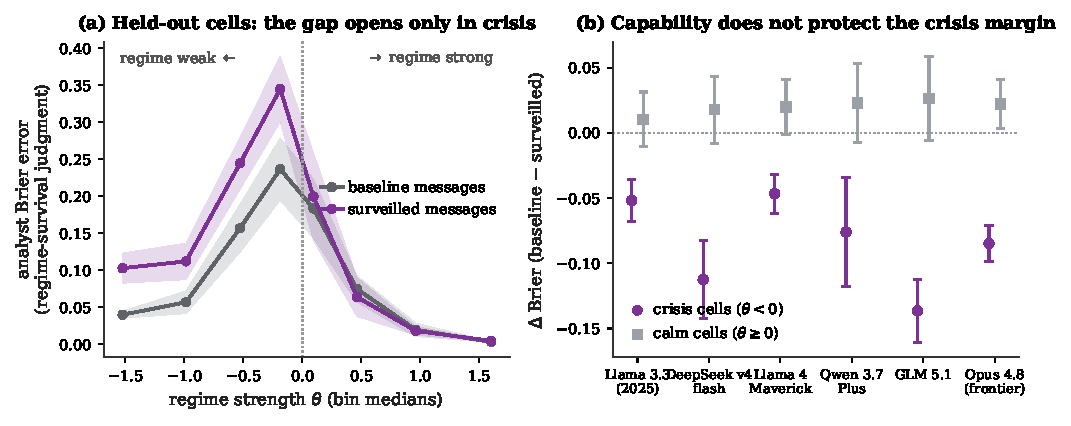
\includegraphics[width=\textwidth]{figures/fig_crisis_blinding.pdf}
\caption{\textbf{Crisis blindness.} (a) Analyst Brier error on regime survival by state, pooled over the four held-out analysts (348 preregistered fresh cells; cell-level 95\% bands). The arms coincide for $\theta \ge 0$ and diverge below it---and the gap peaks not in hopeless states, which are easy to call even from guarded text, but in the \emph{ambiguous tipping-point band}, exactly where the regime's response decision has value. (b) Paired crisis (purple) and calm (gray) Brier deltas by analyst, ordered by capability tier, on the main 150-cell sample. The frontier model loses as much in crisis as models costing two orders of magnitude less.}
\label{fig:crisis}
\end{figure}

Figure~\ref{fig:crisis}(a) shows the result's structure. The blinding is not a uniform haze: surveilled and free traffic are equally readable in strong states and in hopelessly weak ones, and the gap concentrates in the band where the outcome hangs on coordination---the precise region where preemption and concession decisions are made.

\subsection{The blindness is in the data, not the reader}

The frontier analyst is the best model on every level metric (e.g., $|\rho(\text{FALL},\theta)| = 0.93$, the highest in the program) and loses as much in crisis as models costing two orders of magnitude less: crisis $\Delta$Brier $-0.085$ ($p<0.001$), crisis sender-accuracy loss $6.5$ points ($p=0.003$), with significant calm-state \emph{reversals}---surveillance improves its calm-state reading, because uniformly guarded quiet is easy to classify. Capability raises the level of intelligence everywhere; it does not protect the crisis margin, because no reader can extract content the senders never encoded.

A supervised classifier (TF-IDF + logistic regression, cell-level cross-fitting) makes the result model-free: trained on free speech, its sender-level AUC falls from $0.922$ to $0.844$ on surveilled crisis traffic, double the calm-state gap; granting the regime labeled surveilled data to retrain on---the best case, and precisely the data \citet{yang2025} shows regimes lack---recovers only part of the loss.

Cross-sender robustness is, if anything, stronger: on a second sender family (Qwen3-30B corpus), pooled sender AUC falls $0.81 \to 0.67$ and $0.89 \to 0.75$ (both $p<0.0001$), crisis sender-accuracy losses reach $17$--$18$ points, and even the aggregate join-share margin---null on the primary corpus---degrades significantly.

\subsection{What survives, and the decomposition of the loss}

Two margins are robust to surveillance. Aggregate temperature: analysts' join-share estimates barely move on the primary corpus (MAE $\approx 0.17$--$0.25$ in both arms)---the regime can still tell that people are unhappy. And within-cell ranking: per-cell ranking AUC of senders is statistically flat across arms in nearly every test (the isolated failure of the v2 gate). The loss concentrates in \emph{between-cell, state-level} discrimination: which cells are dangerous, and whether the state is one in which coordination will tip. Coding hides the fire, not the relative ordering of the people standing near it. This is the politically decisive margin: preemption, concession, and timing all run on tipping-point detection, the object $H(\cdot)$ acts on in \eqref{eq:survival}, and it is the margin Corollary~\ref{cor:trap} says the regime cannot audit from averages.

\section{Mechanism: the text}\label{sec:mechanism}

\paragraph{Universal compliance, selected destruction.} Across 24{,}306 matched messages, a classifier on simple text features separates surveilled from free messages at AUC $0.93$--$0.97$ in \emph{every} sender-signal and state bin: essentially everyone shifts register under a warning. The divergence gradient is nonetheless monotone in the predicted direction (Spearman $\rho = -0.79$, $p=0.02$ across sender-signal bins; $\rho = -0.98$, $p<0.001$ across $\theta$ bins), but its magnitude makes clear that the style response is a trigger, not a margin. The information loss, by contrast, is sharply selected (Section~\ref{sec:results}): a guarded version of ``nothing is happening'' has the same likelihood ratio as its direct counterpart; a guarded version of ``people I trust are ready to move'' does not. This is Lemma~\ref{lem:register} read off the data, and it is why the model needs no coding-choice cutoff.

\begin{figure}[ht]\centering
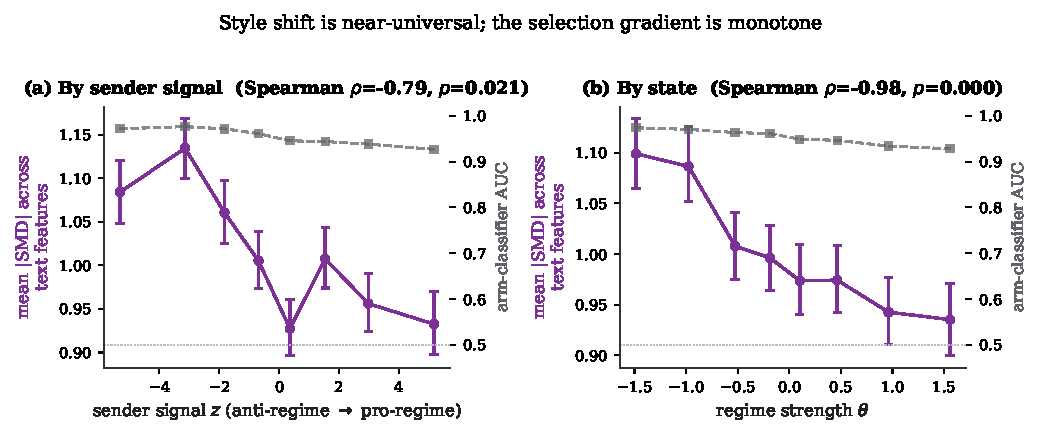
\includegraphics[width=\textwidth]{figures/fig_lemma1_text.pdf}
\caption{\textbf{Universal compliance, selected destruction} (24{,}306 matched messages). Purple: mean absolute standardized difference of text features (action cues, direct regime terms, hedges, commitment language, length) between arms, by sender-signal bin (a) and state bin (b), with bootstrap 95\% CIs. Gray (right axes): AUC of a classifier separating the arms on the same features. The style shift is near-universal---the arms are separable at AUC $0.93$--$0.97$ in every bin---while the divergence gradient is monotone in the predicted direction. The information loss (Figure~\ref{fig:crisis}) is far more selected than the style shift: Lemma~\ref{lem:register}'s structure, read off the text.}
\label{fig:lemma1}
\end{figure}

\paragraph{Style alone is not enough.} On a codedness-control corpus---equally indirect, metaphorical messages elicited \emph{without} monitoring framing---analyst $\theta$-recovery degrades directionally for all three analysts tested but reaches at most marginal significance ($|\rho|$: $0.35$ vs.\ $0.21$, $p=0.06$; $0.44$ vs.\ $0.38$; $0.42$ vs.\ $0.37$). Combined with the companion paper's finding that coded style alone does not move \emph{receivers'} actions, the blinding travels with what monitored senders choose not to convey, more than with indirection as a form.

\section{Dose-response and the regime's problem}\label{sec:dose}

\begin{figure}[ht]\centering
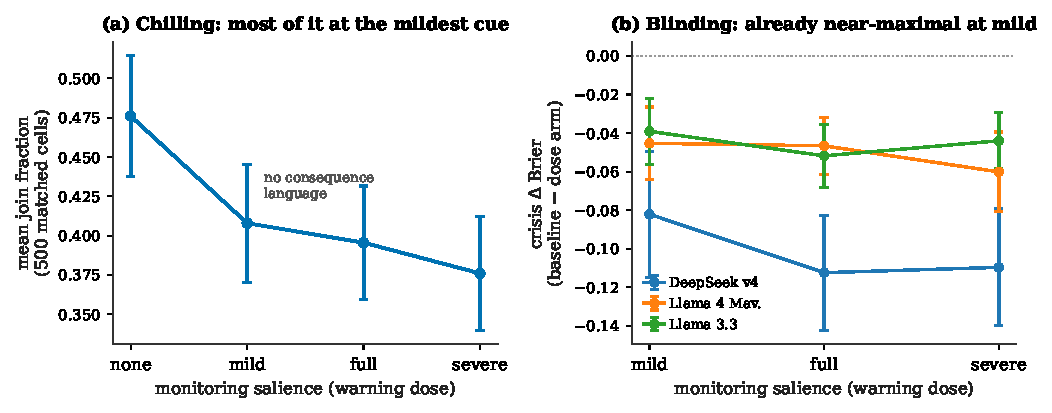
\includegraphics[width=\textwidth]{figures/fig_dose_response.pdf}
\caption{\textbf{Both margins are step functions of monitoring salience.} (a) Mean join fraction across four warning doses on the identical 500-cell grid (cell-level 95\% CIs); the mild cue---``communications are sometimes subject to routine monitoring,'' no consequence language---delivers two-thirds of the total chilling. (b) Crisis-state Brier deltas by dose for three analysts; the mild dose already produces $75$--$85\%$ of full-dose blinding, and severity adds little.}
\label{fig:dose}
\end{figure}

Graded warnings on the identical 500-cell grid trace both curves (Figure~\ref{fig:dose}). Chilling (mean join fraction): none $0.471$, mild $0.408$, full $0.391$, severe $0.376$---monotone, strongly concave, two-thirds of the total at the mildest cue, which contains no consequence language at all. Blinding (crisis $\Delta$Brier, three analysts): the mild dose already delivers $75$--$85\%$ of the full-dose effect (e.g., DeepSeek $-0.082$ mild, $-0.112$ full, $-0.110$ severe; all $p<0.0001$ at every dose). Both effects arrive almost entirely at the extensive margin, supporting the trigger interpretation of compliance (Remark~\ref{rem:uniform}) and the binary statement of the regime's problem (Proposition~\ref{prop:extensive}).

The regime-side implication is uncomfortable for the watcher. Conditional on visible monitoring, more severity is roughly free: extra silence at little extra blindness. But the step from silence to any visible monitoring purchases nearly all the deterrence at nearly all the intelligence cost---and by Corollary~\ref{cor:trap}, the cost is invisible in the regime's own average metrics. \emph{[To add: calibrated survival comparison $S(1)$ vs.\ $S(0)$ using the measured $U$ and $I_R$ curves and a parameterized response function $H$; the exhibit traces the monitor-vs-silent frontier in $(H', G)$ space.]}

\section{Discussion}\label{sec:discussion}

\paragraph{The platform cycle.} Propositions~\ref{prop:twoprices}--\ref{prop:tail} rationalize a familiar arc. A new channel arrives unmonitored; willingness becomes mutually legible; mobilization waves follow. The state learns the channel and advertises monitoring; speech shifts into the guarded register; coordination fails---and the state's own reading of society decays, invisibly, precisely in the states where it matters. Discontent is not destroyed; it is stored in a form neither citizens nor the state can read, until the next unmonitored channel restores legibility all at once, to the regime's maximal surprise. Surveillance controls ignition, not fuel; it suppresses the mean of unrest and fattens its tail. The Stasi's files did not warn it about 1989 \citep{kuran1991}; Nepal's ban did not warn it about Discord.

\paragraph{Positioning.} Relative to \citet{yang2025}: his channel is missingness (posts never written) corrupting machine-learning pipelines; this paper's channel is camouflage (messages written, re-encoded) degrading any reader, microfounded in equilibrium and priced jointly with the citizen side. Relative to the dictator's-dilemma theory \citep{egorov2009, gehlbach2026}: those models have no communication stage; here the opacity is produced by the monitoring instrument itself, with a measured dose-response. Relative to information design in regime change \citep{edmond2013, inostroza2025}: manipulation here is horizontal in origin---the regime never touches the receiver's signal structure; it changes the incentives under which peers write, and is itself a victim of the result. The AI-safety parallel \citep{baker2025} is exact in mechanism and worth stating plainly: monitoring pressure selects for less monitorable communication, whether the monitored are citizens or chains of thought; ``monitorability taxes'' are the alignment community's name for the intelligence cost of surveillance.

\paragraph{Limitations.} The agents are language models, not humans; the claims are about the informativeness of message distributions under specified incentives, validated by preregistration, held-out replication, placebo states, cross-model and cross-sender robustness, and a model-free classifier---not by claimed human equivalence. The senders' guarded register may partly reflect alignment training; the codedness control and the universal-compliance pattern bound, but do not eliminate, this concern. The game is static; repeated play could let receivers learn to decode (an euphemism treadmill) and lets grievance accumulate (Proposition~\ref{prop:tail}'s dynamics), both left to future work. And the regime's response function $H$ is calibrated, not derived; endogenizing the response (and the visibility choice as a signaling problem) is the natural next model.

\paragraph{Conclusion.} The paper's accounting identity is simple. Visible surveillance buys silence and pays in blindness; the purchase clears at the mildest visible cue; and the bill is presented in the regime's worst state of the world. The same change in speech that stops citizens from reading each other stops the regime from reading the street. A state that wants to be feared must accept being deceived---not by lies, but by the guarded truth it taught its citizens to tell.

\bibliographystyle{plainnat}
\bibliography{references2,../paper/references}

\end{document}
